\chapter{Networks}

Like humans are mammals, electric cicuits are networks. As such we can learn some important ideas about circuits by first thinking a little bit about networks. \par

We have another motive for studying other networks. Electric circuits involve quantities that are difficult to picture. In order to form a decent mental picture of how they work, it can be useful to make analogies with networks that are easier to picture.\par

\begin{figure}[H]
\begin{center}
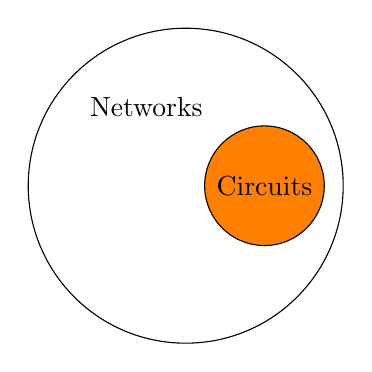
\begin{tikzpicture}
\node[draw,circle,minimum size =4cm] (A) at (0,0){};
\node[draw,circle,minimum size =1cm, fill=orange] (B) at (1,0){Circuits};
\node at (-.5,1) {Networks};
\end{tikzpicture}
\caption{Circuits are Networks}
\label{F:1FCAREN}
\end{center}
\end{figure}

In this first chapter, we take a tour of some other networks and with a mind on what we can apply to electrical networks (circuits). Starting in the next chapter, we'll devote ourselves more wholely to electric networks in particular.\par

\begin{bigidea} 
Electrical circuits are networks. They have a lot in common with other networks.
\end{bigidea}

\begin{bigidea} 
If you want to learn a specific, study the general. For example, if you want to learn about dogs, study mammals. See how dogs differ from racoons or kangaroos. 
\end{bigidea}

\section{Network Examples}

\subsection{A Network of Friends}
The diagram below shows a network of friends.

\begin{figure}[H]
\begin{center}
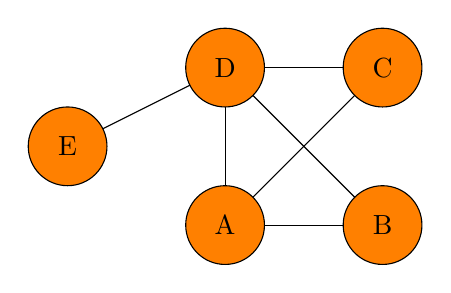
\begin{tikzpicture}
\draw (0,.5)--(0,1.5);
\draw (.5,2)--(1.5,2);
\draw (0,2)--(-2,1);
\draw (0,2)--(2,0);
\draw (0,0)--(2,0);
\draw (0,0)--(2,2);
\node[draw,circle,minimum size =1cm, fill=orange] (A) at (0,0){A};
\node[draw,circle,minimum size =1cm, fill=orange] (B) at (2,0){B};
\node[draw,circle,minimum size =1cm, fill=orange] (C) at (2,2){C};
\node[draw,circle,minimum size =1cm, fill=orange] (D) at (0,2){D};
\node[draw,circle,minimum size =1cm, fill=orange] (E) at (-2,1){E};
\end{tikzpicture}
\caption{A Friends Network}
\label{F:1FN}
\end{center}
\end{figure}

\par
\begin{alevel}
Who has the most friends?
\end{alevel}
\begin{alevel}
Draw a friend network that consists of 4 people where everybody has exactly two friends.
\end{alevel}
\par

\noindent
Networks have \textbf{nodes} and \textbf{edges}. The network in Figure~\ref{F:1FN} has 5 nodes. The edges connect nodes.  The meaning of the edges and node depends on the network. In our friend network, nodes represent people and edges represent relationships. For our friend network shown in Figure~\ref{F:1FN}, the edges have no direction to them. If A were friends with B, then B would be friends with A. However, this wouldn't have to be the case. We could add some directionality to the edges, like in the modified friends network shown in Figure~\ref{F:1FNb}:\\

\begin{figure}[H]
\begin{center}
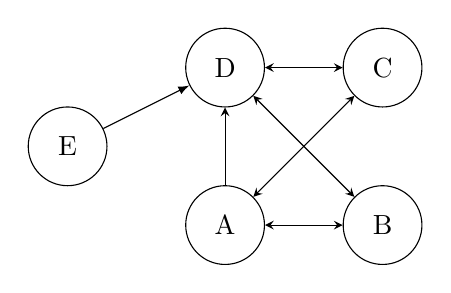
\begin{tikzpicture}
\node[draw,circle,minimum size =1cm] (A) at (0,0){A};
\node[draw,circle,minimum size =1cm] (B) at (2,0){B};
\node[draw,circle,minimum size =1cm] (C) at (2,2){C};
\node[draw,circle,minimum size =1cm] (D) at (0,2){D};
\node[draw,circle,minimum size =1cm] (E) at (-2,1){E};
\draw [stealth-stealth](A) edge (B);
\draw [stealth-stealth](C) edge (A);
\draw [-stealth](A) edge (D);
\draw [latex-](D) edge (E);
\draw [stealth-stealth](D) edge (C);
\draw [stealth-stealth](D) edge (B);
\end{tikzpicture}
\caption{Friends Network with Directional Edges}
\label{F:1FNb}
\end{center}
\end{figure}
\par

\noindent
If an arrow points only from A to B, then A is friends with B but that B is not friends with A. A bidirectional arrow means both people are friends with each other.\par

\begin{alevel}
How many people is D friends with?
\end{alevel}

\subsection{Road Networks}
Consider the road network shown in Figure~\ref{F:1RN} showing 5 towns connected together. The towns are called A, B, C, D and E. Each edge represents a road.\par
\begin{figure}[H]
\begin{center}
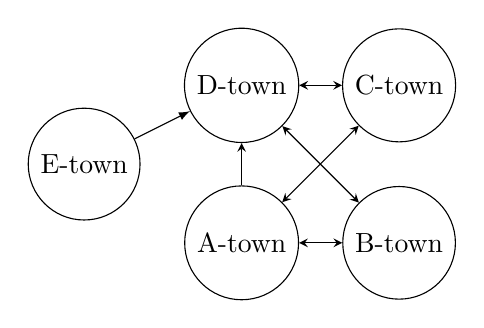
\begin{tikzpicture}
\node[draw,circle,minimum size =1cm] (A) at (0,0){A-town};
\node[draw,circle,minimum size =1cm] (B) at (2,0){B-town};
\node[draw,circle,minimum size =1cm] (C) at (2,2){C-town};
\node[draw,circle,minimum size =1cm] (D) at (0,2){D-town};
\node[draw,circle,minimum size =1cm] (E) at (-2,1){E-town};
\draw [stealth-stealth](A) edge (B);
\draw [stealth-stealth](C) edge (A);
\draw [-stealth](A) edge (D);
\draw [latex-](D) edge (E);
\draw [stealth-stealth](D) edge (C);
\draw [stealth-stealth](D) edge (B);
\end{tikzpicture}
\caption{Road Network}
\label{F:1RN}
\end{center}
\end{figure}

\begin{alevel}
For figure~\ref{F:1RN}, what does each node represent?
\end{alevel}

\begin{alevel}
How many roads are there?
\end{alevel}

\begin{alevel}
What does each edge represent?
\end{alevel}

\begin{alevel}
If each two-way road has two lanes and each one way road has one lane, how many lanes of road does the network have?
\end{alevel}

\begin{alevel}
If you start your trip at B-town, which town(s) can you not get to? If there are more than one, list them all.
\end{alevel}

\begin{clevel}
If you start your trip at E-town, is it possible to reach all the towns without traversing the same road twice? Does the answer to this question depend on the town where you start?
\end{clevel}

\begin{dlevel}
What would need to be true about ANY road network (all two way roads) such that you could always start at any town, travel some combination of roads, and reach every town without traversing any road twice?
\end{dlevel}

A road network diagram might convey more information. The edges could have a length (and/or width) associated with them. Figure~\ref{F:1RNb} shows a road network with the road length information added. 

\par
\begin{figure}[H]
\begin{center}
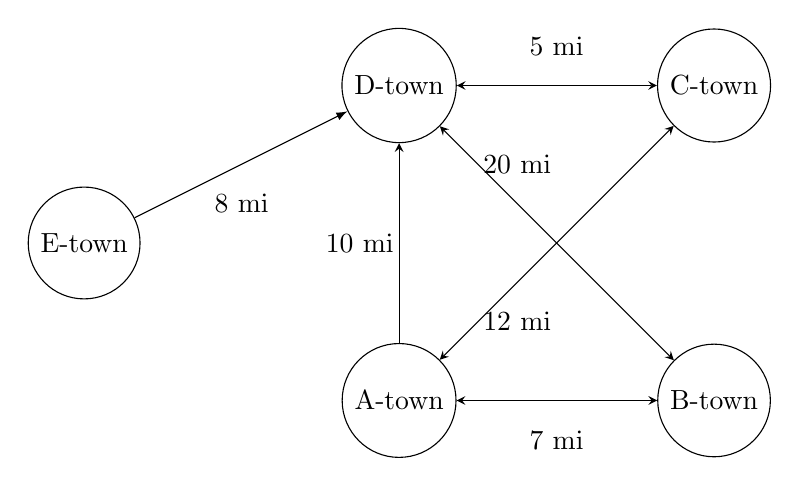
\begin{tikzpicture}
\node[draw,circle,minimum size =1cm] (A) at (0,0){A-town};
\node[draw,circle,minimum size =1cm] (B) at (4,0){B-town};
\node[draw,circle,minimum size =1cm] (C) at (4,4){C-town};
\node[draw,circle,minimum size =1cm] (D) at (0,4){D-town};
\node[draw,circle,minimum size =1cm] (E) at (-4,2){E-town};
\draw [stealth-stealth](A) edge (B);
\node at (2,-.5) {7 mi};
\draw [stealth-stealth](C) edge (A);
\node at (1.5,1) {12 mi};
\draw [-stealth](A) edge (D);
\node at (-.5,2) {10 mi};
\draw [latex-](D) edge (E);
\node at (-2,2.5) {8 mi};
\draw [stealth-stealth](D) edge (C);
\node at (2,4.5) {5 mi};
\draw [stealth-stealth](D) edge (B);
\node at (1.5,3) {20 mi};
\end{tikzpicture}
\caption{Road Network with edges that have values}
\label{F:1RNb}
\end{center}
\end{figure}

\begin{alevel}
What is the shortest distance to travel from E-Town to B-town?
\end{alevel}
\begin{alevel}
Name any node in this network.
\end{alevel}
\noindent
Now suppose there is some traffic on the network. \emph{Something} is flowing along the edges of the network - cars. Suppose there are:
\begin{enumerate}
\item 100 cars/minute flowing from E-town to D-town.  
\item 200 cars/minute (net) flowing from D-town to B-town
\item 50 cars/minute flowing from A-town to D-town
\item D-town and A-town and B-town have no parking at all, anywhere, zip, nada, none. If a town has no parking, the number of cars entering a town \textbf{must} equal the number of cars leaving.
\end{enumerate}

\begin{bigidea} 
Some networks are such that the \emph{flow} into a node must equal the \emph{flow} out of a node.
\end{bigidea}

\begin{alevel}
How many cars per minute must be driving along the road from B-town to A-town?
\end{alevel}

\begin{clevel}
How many cars per minute must be entering C-town?
\end{clevel}

\begin{dlevel}
Describe an algorithm to answer questions like the previous one.
\end{dlevel}

\noindent
Note that two of the roads seem to cross each other. Maybe they intersect there, maybe not. In this book, on a diagram, there is not an intersection unless the figure indicates one \footnote{Or unless it is obvious. Yikes! I realize this is disheartening because when you are new to something, very little seems obvious.}. A dot indicates an intersection, like in Figure~\ref{F:1RNb}.\par
\par
\begin{figure}[H]
\begin{center}
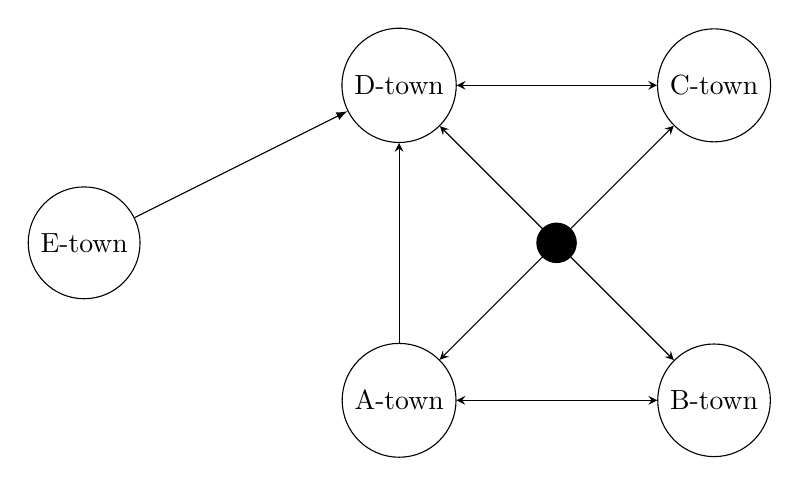
\begin{tikzpicture}
\node[draw,circle,minimum size =1cm] (A) at (0,0){A-town};
\node[draw,circle,minimum size =1cm] (B) at (4,0){B-town};
\node[draw,circle,minimum size =1cm] (C) at (4,4){C-town};
\node[draw,circle,minimum size =1cm] (D) at (0,4){D-town};
\node[draw,circle,minimum size =1cm] (E) at (-4,2){E-town};
\draw [stealth-stealth](A) edge (B);
\draw [stealth-stealth](C) edge (A);
\draw [-stealth](A) edge (D);
\draw [latex-](D) edge (E);
\draw [stealth-stealth](D) edge (C);
\draw [stealth-stealth](D) edge (B);
\node[draw, circle, minimum size=0.5cm, fill=black] at (2,2) {};
\end{tikzpicture}
\caption{Road network with an intersection indicated between Road AC and Road DB.}
\label{F:1RNb}
\end{center}
\end{figure}
\par

\subsection{Water Networks}
Consider the water network shown in Figure~\ref{F:1WN}.\\

\begin{figure}[H]
\begin{center}
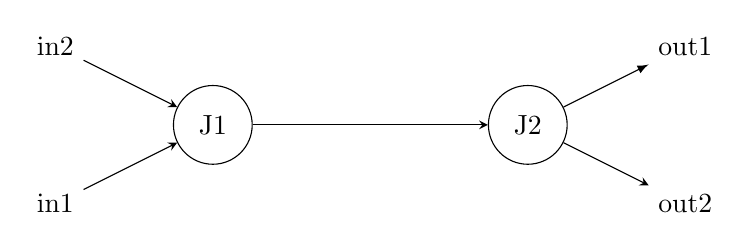
\begin{tikzpicture}
\node (In1) at (0,0){in1};
\node (In2) at (0,2){in2};
\node[draw,circle,minimum size =1cm] (J1) at (2,1){J1};
\node[draw,circle,minimum size =1cm] (J2) at (6,1){J2};
\node (Out1) at (8,2){out1};
\node (Out2) at (8,0){out2};
\draw [-stealth](In1) edge (J1);
\draw [-stealth](In2) edge (J1);
\draw [-stealth](J1) edge (J2);
\draw [-latex](J2) edge (Out1);
\draw [-stealth](J2) edge (Out2);
\end{tikzpicture}
\caption{Water Network}
\label{F:1WN}
\end{center}
\end{figure}

As with any network, you should begin by asking: What do the edges and nodes represent? For this water network\footnote{You might define things a little differently, but it doesn't matter here.}:
\begin{itemize}
\item Each of the \textbf{edges} represents a pipe or hose. Water flows along the edges.
\item Each of the \textbf{nodes} represents a junction, an input or an output. In1 and J2 are example of nodes.
\end{itemize}
What is flowing along the edges? Water.
How should we measure it? Hmmm. Maybe gallons per second (gps) or kg per second, or cubic meters per hour. Let's use gps.

\begin{blevel}
Ten gallons per second (gps) of water comes out the end of a hose. How many kg per second of water is this equivalent to?
\end{blevel}

\begin{blevel}
Suppose water flowed from in1 to J1 at 5 gps and in2 to J1 at 7 gps. Also suppose the flow from J1 to J2 were 10 gps. What would be happening to the amount of water stored in junction J1? How could this be?
\end{blevel}

\begin{clevel}
A 1cm radius water hose has some water flowing through it at a speed of 2 m/s. How many gallons per minute are flowing down this hose? Hint: Think about how much water passes a point in the hose each minute.
\end{clevel}

\subsection{A Neural Network}
Consider the neural network shown in Figure~\ref{F:1NN}. Each edge has a number (called a weight) associated with it. Each node is little calculator that combines the inputs and their weights to produce an output. For example, the calculation might be to sum the products of the inputs and their weights, and if that exceeds 5, then the output is 1, otherwise it is -1. 

The idea is that output depends on the input. By adjusting the weights this machine can be tuned to give a desired output, like "yes that is a piece of fruit" based on a set of inputs like the pixels in an image.
\begin{figure}[H]
\begin{center}
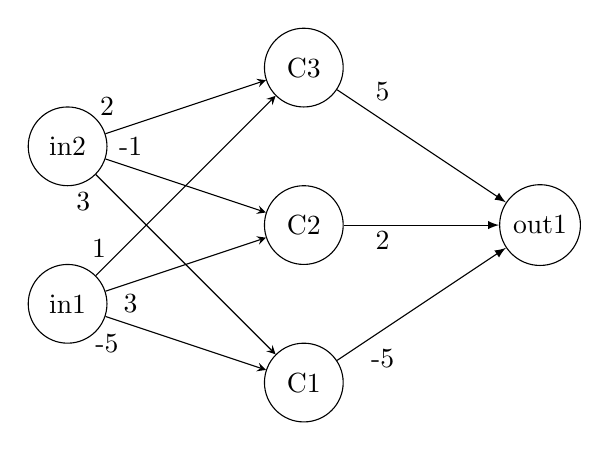
\begin{tikzpicture}
\node [draw,circle,minimum size =1cm](In1) at (0,0){in1};
\node [draw,circle,minimum size =1cm](In2) at (0,2){in2};
\node [draw,circle,minimum size =1cm](C1) at (3,-1){C1};
\node [draw,circle,minimum size =1cm](C2) at (3,1){C2};
\node [draw,circle,minimum size =1cm](C3) at (3,3){C3};
\node [draw,circle,minimum size =1cm](Out1) at (6,1){out1};
\draw [-stealth](In1) edge (C1);
\node at (.5,2.5) {2};
\draw [-stealth](In1) edge (C2);
\node at (.8,2) {-1};
\draw [-stealth](In1) edge (C3);
\node at (.2,1.3) {3};
\draw [-stealth](In2) edge (C1);
\node at (.4,0.7) {1};
\draw [-stealth](In2) edge (C2);
\node at (.8,0) {3};
\draw [-stealth](In2) edge (C3);
\node at (.5,-.5) {-5};
\draw [-latex](C1) edge (Out1);
\node at (4,2.7) {5};
\draw [-latex](C2) edge (Out1);
\node at (4,0.8) {2};
\draw [-latex](C3) edge (Out1);
\node at (4,-.7) {-5};
\end{tikzpicture}
\caption{A Neural Network}
\label{F:1NN}
\end{center}
\end{figure}

\begin{alevel}
For the neural network, what do the nodes represent?
\end{alevel}

\begin{blevel}
Suppose in1 were a 5 and in2 were a 10. What would be the output of C3? Hint: the output of C2 would be 1 because $-1*5+3*10 > 5$.
\end{blevel}

\begin{clevel}
If the output node contained the same calculating machines as the C-nodes, what would be the ouput if in1 were a 5 and in2 were a 10? 
\end{clevel}

\begin{clevel}
Let's call the product of the weight and the value on an edge the \em{flow}. Is it true that the flow into a node must equal the flow out of that node? 
\end{clevel}

\subsection{Summary}
In this section, we browsed some common networks. Let's see what we can takeaway:
\begin{itemize}
\item All networks have edges and nodes.
\item For some networks, the edges have values associated with them.
\item For some networks, the edges can be associated with a flow of something on them.
\item For some networks, the flow into a node must equal the flow out of a node. For other networks, this might not need to be the case.
\item A network might have a useful property, like all nodes have the same number of edges that touch them. Or all edge values are positive, or edges have a direction to them, or something else. Identifying such properties, if they exist, goes a long way towards understanding that particular network.
\end{itemize}



